\documentclass[12pt]{article}

\title{\vspace{-3em}PHYS 167b HW 06}
\author{Michael Cardiff}
\date{\today}

%% science symbols
\usepackage{amsmath}
\usepackage{amssymb}
\usepackage{amsthm}
\usepackage{bm}
\usepackage{cancel}
\usepackage{physics}
\usepackage{siunitx}
\usepackage{slashed}

%% general pretty stuff
\usepackage{caption}
\usepackage{float}
\usepackage{graphicx}
\usepackage{url}
\usepackage{enumitem}
\usepackage{hyperref}
\usepackage{booktabs}
\usepackage{tikz}
\usepackage{tikz-feynhand}

% setup options
\captionsetup{labelfont=bf}
\graphicspath{ {./figs/} }

% macros
\renewcommand{\L}{\mathcal{L}}
\renewcommand{\H}{\mathcal{H}}
\renewcommand{\l}{\ell}
\newcommand{\M}{\mathcal{M}}
\newcommand{\mcV}{\mathcal{V}}
\newcommand{\D}{\partial}
\newcommand{\veps}{\varepsilon}
\newcommand{\circled}[1]{\tikz[baseline = (char.base)]{
    \node[shape=circle,draw,inner sep=2pt] (char){#1};}}

% mdframed environments
\usepackage[framemethod=TikZ]{mdframed}
\mdfsetup{skipabove=\topskip,skipbelow=\topskip}
\mdfdefinestyle{defstyle}{%
  linewidth=1pt,
  frametitlerule=true,
  frametitlebackgroundcolor=gray!40,
  backgroundcolor=gray!20,
  innertopmargin=\topskip}

\mdtheorem[style=defstyle]{definition}{Definition}
\mdtheorem[style=defstyle]{theorem}{Theorem}
\mdtheorem[style=defstyle]{problem}{Problem}[section]

\newenvironment{thebook}
{\begin{mdframed}[style=defstyle,frametitle={From the Book}]}{\end{mdframed}}

\begin{document}
\maketitle
\section{Thomson, Problem 10.3}
\begin{problem}
  Find the overall ``color factor'' for $qq\to qq$ if QCD corresponded to a $SU(2)$ color symmetry.
\end{problem}
If we instead had ${SU(2)}_c$, then we would replace the generators for $SU(3)$ in the vertex with the generators for $SU(2)$, which are the Pauli matrices, so we would have in the new vertex:
\begin{align*}
  -\frac12ig_S\sigma^a_{ij}\gamma^\mu
\end{align*}
Hence now there are 2 colors ($r$ and $g$), and 3 ``gluons'' corresponding to $a=1,2,3$. The color factor would be the same as in the book but with our new generators, giving the constraint of $i,j,k,l=1,2$:
\begin{align*}
  C(ik\to jl)=\frac14\sum_{a=1}^3\sigma^a_{ji}\sigma^a_{kl}
\end{align*}
Similarly, we have several cases for the colors, lets list them out:
\begin{table}[H]
  \centering
  \begin{tabular}{cccc}
    ${\color{blue}rr\to rr}$ & ${\color{red}rr\to rg}$
    &${\color{red}rr\to gg}$ & ${\color{red}rr\to gr}$\\\midrule
    ${\color{red}rg\to rr}$ & ${\color{blue}rg\to rg}$
    & ${\color{red}rg\to gg}$ & ${\color{blue}rg\to gr}$\\\midrule
    ${\color{red}gg\to rr}$ & ${\color{red}gg\to rg}$ 
    & ${\color{blue}gg\to gg}$ & ${\color{red}gg\to gr}$\\\midrule
    ${\color{red}gr\to rr}$ & ${\color{blue}gr\to rg}$ 
    & ${\color{red}gr\to gg}$ & ${\color{blue}gr\to gr}$
  \end{tabular}
  \caption{Color Combinations for ${SU(2)}_c$}
\end{table}
Note, only the {\color{blue}blue} ones conserve color, so they will be the only nonzero elements, hence we only need to find:
\begin{align*}
  C(rr\to rr)\quad C(gg\to gg)\\
  C(rg\to rg)\quad C(gr\to gr)\\
  C(rg\to gr)\quad C(gr\to rg)
\end{align*}
Where factors on the same row should be the same, hence, looking at the elements of the Pauli matrices we can find that:
\begin{align*}
  C(rr\to rr)=C(gg\to gg)&=\frac14(+1)(+1)=+\frac14\\
  C(rg\to rg)=C(gr\to gr)&=\frac14(+1)(-1)=-\frac14\\
  C(rg\to gr)=C(gr\to rg)&=\frac14\qty[(+1)(+1)+(+i)(-i)]=\frac12
\end{align*}
Now we need to average over all the combinations, accounting for the 4 initial color combinations, we find that:
\begin{align*}
  \ev{\abs{C}^2}=\frac14\sum_{i,j,k,l}\abs{C(ij\to kl)}^2
\end{align*}
Noting we have 2 of each of the non-zero factors, we find:
\begin{align*}
  \ev{\abs{C}^2}=\frac12
  \qty[{\qty(\frac14)}^2+{\qty(\frac14)}^2+{\qty(\frac12)}^2]
  =\frac3{16}
\end{align*}
Hence if we instead have an ${SU(2)}_c$, the color factor would be:
\begin{equation}
  \label{eq:p1}
  \boxed{\ev{\abs{C}^2}=\frac3{16}}
\end{equation}
\newpage
\section{Thomson, Problem 11.1}
\begin{problem}
  Explain why the strong decay $\rho^0\to\pi^-\pi^+$ is observed, but the strong decay $\rho^0\to\pi^0\pi^0$ is not.

  Hint: you will need to consider conservation of angular momentum, parity, and the symmetry of the $\pi^0\pi^0$ wavefunction.
\end{problem}
From the PDG, we can see that $J^P$ for the pions is $J^P=0^-$, and for $\rho^0$ we have $J^P=1^-$, meaning in order for angular momentum to be conserved, the $\pi$ particles must have orbital angular momentum to decay, specifically in the $L=1$ state. This ensures that parity is conserved as well, as the negative parity of the $\pi$'s will cancel out, leaving only the contribution from the $\ell=1$:
\begin{align*}
  -1=(-1)\times(-1)\times{(-1)}^1=-1
\end{align*}
However, the case with $\pi^0\pi^0$ is different, as there are two identical particles in the final state. This means the overall wavefunction needs to be symmetric. Since the pion's flavor, spin, and color wavefunctions are all symmetric, the antisymmetric $\ell=1$ state (under exchange of the $\pi^0$) makes this an impossible decay
\newpage
\section{Thomson, Problem 11.5}
\begin{problem}
  Consider the decay at rest $\tau^-\to\pi^-\nu_\tau$, where the spin of the tau is in the positive $z$-direction and the $\nu_\tau$ and $\pi^-$ travel in the $\pm z$-directions.  Sketch the allowed spin configurations assuming that the form of the weak charged-current interaction is (i) $V-A$ and (ii) $V+A$.
\end{problem}
The only particle we need to consider the spin of is the neutrino, since the pion has spin 0.
\begin{enumerate}[label = (\roman*)]
\item The $V-A$ interaction corresponds to a $P_L$ operator in the interaction vertex, so only LH chiral particle states are allowed, and the neutrino is kinematically massless, so its spin state is essentially its chiral state, hence:
  \begin{figure}[H]
    \centering
    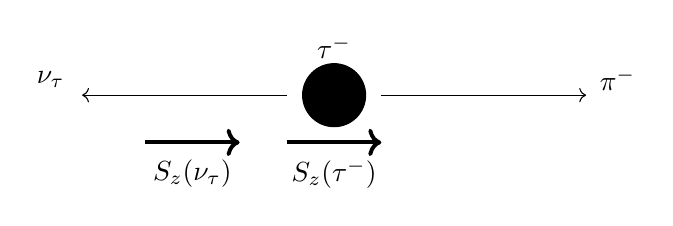
\begin{tikzpicture}[scale=2.0]
      \node (n1) at (0,0.3) {\(\tau^-\)};
      \draw[fill] (0,0) circle (0.2);
      \node (n2) at (1.8,0.1) {\(\pi^-\)};
      \draw[->] (0.3,0) -> (1.6,0);
      \node (n3) at (-1.8,0.1) {\(\nu_\tau\)};
      \draw[->] (-0.3,0) -> (-1.6,0);
      \node (n4) at (-0.9,-0.5) {\(S_z(\nu_\tau)\)};
      \draw[<-, line width=0.5mm] (-0.6,-0.3) -> (-1.2,-0.3);
      \node (n5) at (0.0,-0.5) {\(S_z(\tau^-)\)};
      \draw[->, line width=0.5mm] (-0.3,-0.3) -> (0.3,-0.3);
    \end{tikzpicture}
    \caption{Spin Configurations for $V-A$}\label{fig:p3a}
  \end{figure}
  Where the arrows coming out from the center represent momentum direction, and the lower arrows represent spin
\item The $V+A$ interaction introduces a $P_R$ on the contrary, so instead the neutrino needs to be a RH chiral particle:
  \begin{figure}[H]
    \centering
    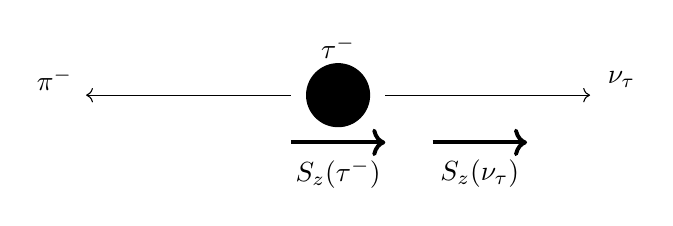
\begin{tikzpicture}[scale=2.0]
      \node (n1) at (0,0.3) {\(\tau^-\)};
      \draw[fill] (0,0) circle (0.2);
      \node (n2) at (1.8,0.1) {\(\nu_\tau\)};
      \draw[->] (0.3,0) -> (1.6,0);
      \node (n3) at (-1.8,0.1) {\(\pi^-\)};
      \draw[->] (-0.3,0) -> (-1.6,0);
      \node (n4) at (0.9,-0.5) {\(S_z(\nu_\tau)\)};
      \draw[->, line width=0.5mm] (0.6,-0.3) -> (1.2,-0.3);
      \node (n5) at (0.0,-0.5) {\(S_z(\tau^-)\)};
      \draw[->, line width=0.5mm] (-0.3,-0.3) -> (0.3,-0.3);
    \end{tikzpicture}
    \caption{Spin Configurations for $V+A$}\label{fig:p3b}
  \end{figure}
\end{enumerate}
\newpage
\section{Thomson, Problem 11.4}
\begin{problem}
  In the annihilation process $e^+e^-\to  q\overline{q}$, the QED vector interaction leads to non-zero matrix elements only for the chiral combinations $LR\to LR$, $LR\to RL$, $RL\to RL$, $RL\to LR$. What are the corresponding allowed chiral combinations for $S,P$ and $S-P$ interactions?
\end{problem}
First consider the $S$ interaction, where the interaction current is simply $\overline{\psi}_1\psi_2$. First consider the LR current:
\begin{align*}
  \overline{v}_L u_R={(P_R v_L)}^\dag\gamma^0P_R u_R
  =v_L^\dag P_R^\dag\gamma^0P_R u_R
\end{align*}
Then noting the form of $P_R$ and the properties of $\gamma^5$:
\begin{align*}
  P_R^\dag\propto{(1+\gamma^5)}^\dag=1+\gamma^5
\end{align*}
Then since $\gamma^5$ anticommutes with $\gamma^0$, we get:
\begin{align*}
  v_L^\dag P_R^\dag\gamma^0P_R u_R=
  \frac14\overline{v}_L(1-\gamma^5)(1+\gamma^5)u_R=
  \overline{v}_L P_L P_R u_R=0
\end{align*}
We can then deduce which currents will not be 0. We need to have opposite projectors on the antiparticle and particle. Which means their chiral states need to align, since the projectors are opposite for the antiparticles, hence the allowed combinations are:
\begin{equation}
  \label{eq:p4a}
  \boxed{LL\to LL,\, LL\to RR,\, RR\to LL,\, \text{ and } RR\to RR}
\end{equation}
For a $P$ interaction, we need not do any more work, since we will have the exact same situation as we did for the $S$ interaction, since the $\gamma^5$ in the Pseudoscalar bilinear commutes with all terms in the projectors, so we once again have
\begin{equation}
  \label{eq:p4b}
  \boxed{LL\to LL,\, LL\to RR,\, RR\to LL,\, \text{ and } RR\to RR}
\end{equation}
For an $S-P$ interaction, we essentially have an extra factor of $P_L$ in our currents, so we can no longer have ANY right handed chiralities in the initial state. As for the final state, the $P_L$ projects out any left handed antiparticles, so we only have one remaining possibility:
\begin{equation}
  \label{eq:p4c}
  \boxed{LL\to RR}
\end{equation}
\newpage
\section{Thomson, Problem 11.10}
\begin{problem}
  Calculate the partial decay width for the decay $\tau^-\to\pi^-\nu_\tau$ in the following steps.
  \begin{enumerate}[label = (\alph*)]
  \item Draw the Feynman diagram and show that the corresponding matrix element is
    \begin{align*}
      \M\approx\sqrt{2}G_F f_\pi\overline{u}(p_\nu)\gamma^\mu
      \frac12(1-\gamma^5)u(p_\tau)g_{\mu\nu}p_\pi^\nu
    \end{align*}
  \end{enumerate}
\end{problem}
First, the diagram:
\begin{figure}[H]
  \centering
  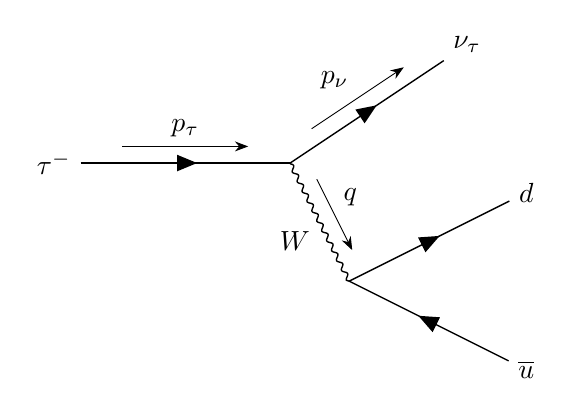
\begin{tikzpicture}[scale=1.5]
    \begin{feynhand}
      % particle positions and whatnot
      \vertex (t) at (0, 0) {$\tau^-$};
      \vertex (n) at (3.5, 1) {$\nu_\tau$};
      \vertex (u) at (4,-1.75) {$\overline{u}$};
      \vertex (d) at (4,-0.25) {$d$};
      \vertex (a) at (2, 0);
      \vertex (b) at (2.5,-1);
      % propagators
      \propag[fer, mom={$p_\tau$}] (t) to (a);
      \propag[fer, mom={$p_\nu$}] (a) to (n);
      \propag[fer] (b) to (d);
      \propag[antfer] (b) to (u);
      \propag[bos, mom={$q$}] (a) to [edge label'=$W$] (b);
    \end{feynhand}
  \end{tikzpicture} 
  \caption{Feynman Diagram for $\tau^-\to\pi^-\nu_\tau$}\label{fig:p5a1}
\end{figure}
However, we want to reduce this a bit (and I assume we do not want to be calculating 3 body phase space), so the better diagram perhaps would be:
\begin{figure}[H]
  \centering
  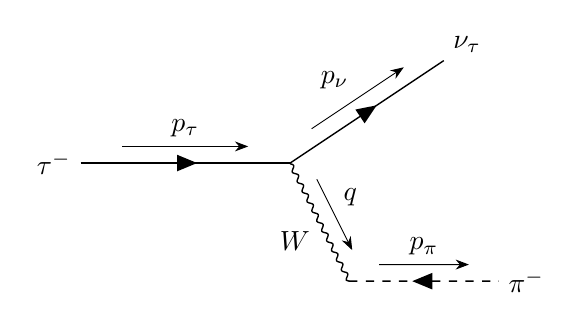
\begin{tikzpicture}[scale=1.5]
    \begin{feynhand}
      % particle positions and whatnot
      \vertex (t) at (0, 0) {$\tau^-$};
      \vertex (n) at (3.5, 1) {$\nu_\tau$};
      \vertex (p) at (4,-1) {$\pi^-$};
      \vertex (a) at (2, 0);
      \vertex (b) at (2.5,-1);
      % propagators
      \propag[fer, mom={$p_\tau$}] (t) to (a);
      \propag[fer, mom={$p_\nu$}] (a) to (n);
      \propag[antsca, mom={$p_\pi$}] (b) to (p);
      \propag[bos, mom={$q$}] (a) to [edge label'=$W$] (b);
    \end{feynhand}
  \end{tikzpicture} 
  \caption{Modified Feynman Diagram for $\tau^-\to\pi^-\nu_\tau$}\label{fig:p5a2}
\end{figure}
This allows us to write the $\pi^-$ weak vertex as $f_\pi p_\pi^\nu$, giving the following form for the matrix element, using the limit where $q^2\ll m_W^2$, which is reasonable as $m_\tau\ll m_W$:
\begin{align*}
  \M=\qty[\frac{g_W}{\sqrt{2}}
  \overline{u}(p_\nu)\gamma^\mu\frac12(1-\gamma^5)u(p_\tau)]\times
  \qty[\frac{g_{\mu\nu}}{m_W^2}]\times
  \qty[\frac{g_W}{2\sqrt{2}}f_\pi p_\pi^\nu]
\end{align*}
Gather factors of two:
\begin{align*}
  \M=\frac{g_W^2}{4m_W^2}
  \overline{u}(p_\nu)\gamma^\mu\frac12(1-\gamma^5)u(p_\tau)
  g_{\mu\nu}f_\pi p_\pi^\nu
\end{align*}
From the definition of $G_F$, we have $\sqrt{2}G_F=g_W^2/4m_W^2$, leaving us with the desired result:
\begin{equation}
  \label{eq:p5a}
  \boxed{\M=\sqrt{2}G_F
  \overline{u}(p_\nu)\gamma^\mu\frac12(1-\gamma^5)u(p_\tau)
  g_{\mu\nu}f_\pi p_\pi^\nu}
\end{equation}
\begin{problem}
  \begin{enumerate}[label = (\alph*)]
    \setcounter{enumi}{1}
  \item Taking the $\tau^-$ spin to be in the $z$-direction and the four-momentum of the neutrino to be:
    \begin{align*}
      p_\nu=p^*(1,\sin\theta,0,\cos\theta)
    \end{align*}
    Show that the leptonic current is
    \begin{align*}
      j^\mu=\sqrt{2m_\tau p^*}(-s,-c,-ic,s)
    \end{align*}
    Note that for this configuration, the spinor for the $\tau^-$ can be taken to be $u_1$ for a particle at rest.
  \end{enumerate}
\end{problem}
Using the note in the problem and the fact that neutrinos are kinematically massess, we can use the left-handed chiral (helicity) state for $\overline{u}(p_\nu)$:
\begin{align*}
  j^\mu=u^\dag_\downarrow(p_\nu)\gamma^0\gamma^\mu u_1(p_\tau)
\end{align*}
The spinors we need to use are:
\begin{align*}
  u_\downarrow=\sqrt{p^*}\pmqty{-s\\c\\s\\-c}\quad\text{and}\quad
  u_1=\sqrt{2m_\tau}\pmqty{1\\0\\0\\0}
\end{align*}
Performing the individual calculations:
\begin{align*}
  j^0&=\sqrt{2m_\tau p^*}\spmqty{-s&c&s&-c}
  \spmqty{1\\&1\\&&-1\\&&&-1}\spmqty{1\\&1\\&&-1\\&&&-1}
  \spmqty{1\\0\\0\\0}=\sqrt{2m_\tau p^*}(-s)\\
  j^1&=\sqrt{2m_\tau p^*}\spmqty{-s&c&s&-c}
  \spmqty{1\\&1\\&&-1\\&&&-1}\spmqty{&&&1\\&&1\\&-1\\-1}
  \spmqty{1\\0\\0\\0}=\sqrt{2m_\tau p^*}(-c)\\
  j^2&=\sqrt{2m_\tau p^*}\spmqty{-s&c&s&-c}
  \spmqty{1\\&1\\&&-1\\&&&-1}\spmqty{&&&-i\\&&i\\&i\\-i}
  \spmqty{1\\0\\0\\0}=\sqrt{2m_\tau p^*}(-ic)\\
  j^3&=\sqrt{2m_\tau p^*}\spmqty{-s&c&s&-c}
  \spmqty{1\\&1\\&&-1\\&&&-1}\spmqty{&&1\\&&&-1\\-1\\&1}
  \spmqty{1\\0\\0\\0}=\sqrt{2m_\tau p^*}(s)
\end{align*}
Or, as described earlier:
\begin{equation}
  \label{eq:p5b}
  \boxed{j^\mu=\sqrt{2m_\tau p^*}(-s,-c,-ic,s)}
\end{equation}
\begin{problem}
  \begin{enumerate}[label = (\alph*)]
    \setcounter{enumi}{2}
  \item Write down the four-momentum of the $\pi^-$ and  show that
    \begin{align*}
      \abs{\M}^2=4G_F^2f_\pi^2m_\tau^3p^*\sin^2\frac\theta2
    \end{align*}
  \end{enumerate}
\end{problem}
The four-momentum of the pion is not as simple as the neutrino, as its mass is non-negligible, but it is doing to come out opposite the $\nu_\tau$:
\begin{align*}
  p^\nu_\pi=(E_\pi,-p^*\sin\theta,0,-p^*\cos\theta)
\end{align*}
Write the term involving this which appears in the matrix element, $j\vdot p$:
\begin{align*}
  j\vdot p_\pi=\sqrt{2m_\tau p^*}
  \qty(-E_\pi\sin\frac\theta2
  -p^*\sin\theta\cos\frac\theta2
  +p^*\cos\theta\sin\frac\theta2)
\end{align*}
The two terms with $p^*$ are a simple trig identity which reduces to just $\sin\theta/2$:
\begin{align*}
  j\vdot p_\pi=-\sqrt{2m_\tau p^*}
  \qty(E_\pi+p^*)\sin\frac\theta2
\end{align*}
However, since $E_\nu\approx p^*$ in this limit, conservation of enegy will give $E_\pi+p^*=m_\tau$:
\begin{align*}
  j\vdot p_\pi=-\sqrt{2m_\tau^3 p^*}
  \sin\frac\theta2
\end{align*}
Hence we arrive at:
\begin{equation}
  \label{eq:p5c}
  \boxed{\abs{\M}^2=4G_F^2f_\pi^2m_\tau^3p^*\sin^2\frac\theta2}
\end{equation}
\begin{problem}
  \begin{enumerate}[label = (\alph*)]
    \setcounter{enumi}{3}
  \item Hence show that
    \begin{align*}
      \Gamma(\tau^-\to\pi^-\nu_\tau)=\frac{G_F^2f_\pi^2}{16\pi}m_\tau^3
      {\qty(\frac{m_\tau^2-m_\pi^2}{m_\tau^2})}^2
    \end{align*}
  \end{enumerate}
\end{problem}
Since we did not treat the $\pi^-$ as its quark content, we can instead use the general phase space formula for $\Gamma$ which was derived in chapter 2:
\begin{align*}
  \Gamma=\frac{p^*}{32\pi^2m_\tau^2}\int\abs{\M}^2\dd{\Omega}
\end{align*}
Collecting factors:
\begin{align*}
  \Gamma=\frac{{(p^*)}^2G_F^2f_\pi^2m_\tau}{8\pi^2}
  \int_{-\pi}^\pi\int_0^{2\pi}\sin^2\frac\theta2\sin\theta\dd{\phi}\dd{\theta}
\end{align*}
The integral is evaluated simply:
\begin{align*}
  \int_{-\pi}^\pi\int_0^{2\pi}\sin^2\frac\theta2\sin\theta\dd{\phi}\dd{\theta}
  =2\pi
\end{align*}
Giving:
\begin{align*}
  \Gamma=\frac{{(p^*)}^2G_F^2f_\pi^2m_\tau}{4\pi}
\end{align*}
The formula given for $p^*$ is:
\begin{align*}
  p^*&=\frac1{2m_\tau}
  \sqrt{[m_\tau^2-{(m_\pi+m_\nu)}^2][m_\tau^2-{(m_\pi-m_\nu)}^2]}\\
  &=\frac1{2m_\tau}\sqrt{[m_\tau^2-m_\pi^2][m_\tau^2-m_\pi^2]}\\
  &=\frac{m_\tau^2-m_\pi^2}{2m_\tau}
\end{align*}
Hence we arrive at the desired result after a bit of algebra:
\begin{equation}
  \label{eq:p5d}
  \boxed{\Gamma(\tau^-\to\pi^-\nu_\tau)=\frac{G_F^2f_\pi^2}{16\pi}
  m_\tau^3{\qty(\frac{m_\tau^2-m_\pi^2}{m_\tau^2})}^2}
\end{equation}
\begin{problem}
  \begin{enumerate}[label = (\alph*)]
    \setcounter{enumi}{4}
  \item Using the value of $f_\pi$ obtained in the previous problem, find a numerical value for $\Gamma(\tau^-\to\pi^-\nu_\tau)$
  \end{enumerate}
\end{problem}
The width (in GeV) would be given by taking $f_\pi=m_\pi$:
\begin{equation}
  \label{eq:p5e}
  \boxed{\Gamma(\tau^-\to\pi^-\nu_\tau)\approx\SI{2.9e-13}{GeV}}
\end{equation}
\begin{problem}
  \begin{enumerate}[label = (\alph*)]
    \setcounter{enumi}{5}
  \item Given that the lifetime of the $\tau$-lepton is measured to be $\tau_\tau=\SI{2.906e-13}{s}$, find an approximate value for the $\tau^-\to\pi^-\nu_\tau$ branching ratio.
  \end{enumerate}
\end{problem}
The appropriate conversion factor would be $\Gamma_\tau=\hbar/\tau_\tau$, giving $\Gamma_\tau=\SI{2.3e-12}{GeV}$ and:
\begin{equation}
  \label{eq:p5f}
  \boxed{BR(\tau^-\to\pi^-\nu_\tau)
    =\frac{\SI{2.9e-13}{GeV}}{\SI{2.3e-12}{GeV}}
  \approx12.8\%}
\end{equation}
\newpage
\section{Thomson, Problem 14.1}
\begin{problem}
  Draw the lowest-order Feynman diagrams for the decays
  \begin{align*}
    K^0\to\pi^+\pi^-\quad
    K^0\to\pi^0\pi^0\quad
    \overline{K}^0\to\pi^+\pi^-\quad
    \overline{K}^0\to\pi^0\pi^0
  \end{align*}
  And state how the corresponding matrix elements depend on the Cabibbo angle $\theta_c$
\end{problem}
Noting the quark content of these mesons is:
\begin{table}[H]
  \centering
  \begin{tabular}{cc}
    Meson & Quarks\\\midrule
    $K^0$ & $d\overline{s}$\\
    $\overline{K}^0$ & $s\overline{d}$\\
    $\pi^+$ & $d\overline{u}$\\
    $\pi^0$ & $u\overline{u}$,$d\overline{d}$\\
    $\pi^-$ & $u\overline{d}$
  \end{tabular}
  \caption{Quark content of mesons}\label{tab:mesons}
\end{table}
We can then do each of the diagrams:
\begin{figure}[H]
  \centering
  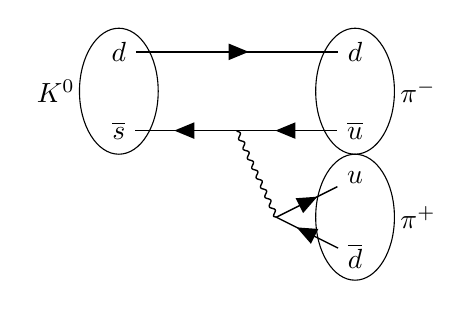
\begin{tikzpicture}
    \node (n1) at (-0.8,-0.5) {\(K^0\)};
    \draw (0,-0.5) ellipse (0.5 and 0.8);
    \node (n2) at (3.8,-0.5) {\(\pi^-\)};
    \draw (3,-0.5) ellipse (0.5 and 0.8);
    \node (n2) at (3.8,-2.1) {\(\pi^+\)};
    \draw (3,-2.1) ellipse (0.5 and 0.8);
    \begin{feynhand}
      % propagated d
      \vertex (d1) at (0,0) {$d$};
      \vertex (d2) at (3,0) {$d$};
      \propag[fer] (d1) to (d2);
      % scattered ~s
      \vertex (s1) at (0,-1) {$\overline{s}$};
      \vertex (a) at (1.5,-1);
      \vertex (s2) at (3,-1) {$\overline{u}$};
      \propag[antfer] (s1) to (a);
      \propag[antfer] (a) to (s2);
      % W decay
      \vertex (b) at (2,-2.1);
      \propag[bos] (a) to (b);
      \vertex (u) at (3,-1.6) {$u$};
      \vertex (db) at (3,-2.6) {$\overline{d}$};
      \propag[fer] (b) to (u);
      \propag[antfer] (b) to (db);
    \end{feynhand}
  \end{tikzpicture}
  \caption{$K^0\to\pi^+\pi^-$}\label{fig:p6a}
\end{figure}
In this diagram, we have two vertices which involve $\theta_C$, one would be $\sin\theta_C$, the other $\cos\theta_C$
\begin{figure}[H]
  \centering
  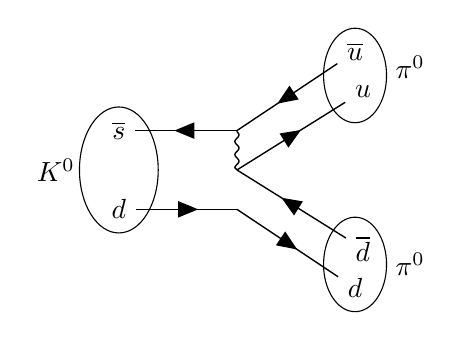
\begin{tikzpicture}
    \node (n1) at (-0.8,-0.5) {\(K^0\)};
    \draw (0,-0.5) ellipse (0.5 and 0.8);
    \node (n2) at (3.7,0.8) {\(\pi^0\)};
    \draw (3,0.7) ellipse (0.4 and 0.6);
    \node (n2) at (3.7,-1.7) {\(\pi^0\)};
    \draw (3,-1.7) ellipse (0.4 and 0.6);
    \begin{feynhand}
      % scattered ~s
      \vertex (s1) at (0,0) {$\overline{s}$};
      \vertex (s2) at (3,1) {$\overline{u}$};
      \vertex (a) at (1.5,0);
      \propag[antfer] (s1) to (a);
      \propag[antfer] (a) to (s2);
      % propagated d
      \vertex (d1) at (0,-1) {$d$};
      \vertex (d2) at (3,-2) {$d$};
      \vertex (c) at (1.5,-1);
      \propag[fer] (d1) to (c);
      \propag[fer] (c) to (d2);
      % W decay
      \vertex (b) at (1.5,-0.5);
      \propag[bos] (a) to (b);
      \vertex (u) at (3.1,0.5) {$u$};
      \vertex (db) at (3.1,-1.5) {$\overline{d}$};
      \propag[fer] (b) to (u);
      \propag[antfer] (b) to (db);
    \end{feynhand}
  \end{tikzpicture}
  \caption{$K^0\to\pi^0\pi^0$}\label{fig:p6b}
\end{figure}
Which has the same dependence on $\theta_C$ as the previous diagram. The $\overline{K}^0$ decays have two similar diagrams:
\begin{figure}[H]
  \centering
  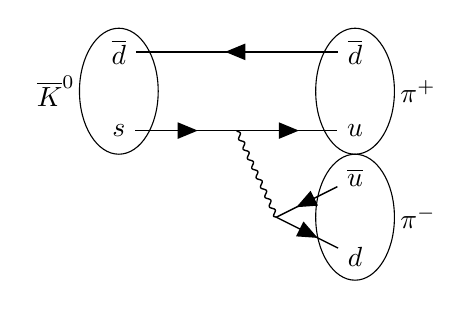
\begin{tikzpicture}
    \node (n1) at (-0.8,-0.5) {\(\overline{K}^0\)};
    \draw (0,-0.5) ellipse (0.5 and 0.8);
    \node (n2) at (3.8,-0.5) {\(\pi^+\)};
    \draw (3,-0.5) ellipse (0.5 and 0.8);
    \node (n2) at (3.8,-2.1) {\(\pi^-\)};
    \draw (3,-2.1) ellipse (0.5 and 0.8);
    \begin{feynhand}
      % propagated d
      \vertex (d1) at (0,0) {$\overline{d}$};
      \vertex (d2) at (3,0) {$\overline{d}$};
      \propag[antfer] (d1) to (d2);
      % scattered ~s
      \vertex (s1) at (0,-1) {$s$};
      \vertex (a) at (1.5,-1);
      \vertex (s2) at (3,-1) {$u$};
      \propag[fer] (s1) to (a);
      \propag[fer] (a) to (s2);
      % W decay
      \vertex (b) at (2,-2.1);
      \propag[bos] (a) to (b);
      \vertex (u) at (3,-1.6) {$\overline{u}$};
      \vertex (db) at (3,-2.6) {$d$};
      \propag[antfer] (b) to (u);
      \propag[fer] (b) to (db);
    \end{feynhand}
  \end{tikzpicture}
  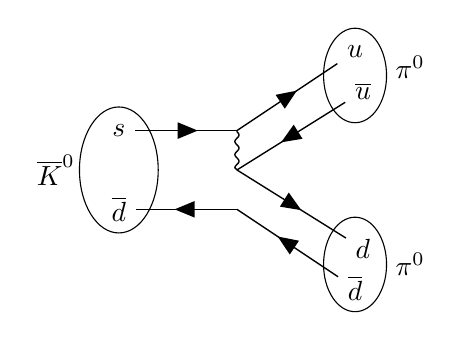
\begin{tikzpicture}
    \node (n1) at (-0.8,-0.5) {\(\overline{K}^0\)};
    \draw (0,-0.5) ellipse (0.5 and 0.8);
    \node (n2) at (3.7,0.8) {\(\pi^0\)};
    \draw (3,0.7) ellipse (0.4 and 0.6);
    \node (n2) at (3.7,-1.7) {\(\pi^0\)};
    \draw (3,-1.7) ellipse (0.4 and 0.6);
    \begin{feynhand}
      % scattered ~s
      \vertex (s1) at (0,0) {$s$};
      \vertex (s2) at (3,1) {$u$};
      \vertex (a) at (1.5,0);
      \propag[fer] (s1) to (a);
      \propag[fer] (a) to (s2);
      % propagated d
      \vertex (d1) at (0,-1) {$\overline{d}$};
      \vertex (d2) at (3,-2) {$\overline{d}$};
      \vertex (c) at (1.5,-1);
      \propag[antfer] (d1) to (c);
      \propag[antfer] (c) to (d2);
      % W decay
      \vertex (b) at (1.5,-0.5);
      \propag[bos] (a) to (b);
      \vertex (u) at (3.1,0.5) {$\overline{u}$};
      \vertex (db) at (3.1,-1.5) {$d$};
      \propag[antfer] (b) to (u);
      \propag[fer] (b) to (db);
    \end{feynhand}
  \end{tikzpicture}
  \caption{$\overline{K}^0\to\pi^+\pi^-$ and $\overline{K}^0\to\pi^0\pi^0$}\label{fig:p6c}
\end{figure}
Which both also have the same $\theta_C$ dependence, hence, for all of these diagrams:
\begin{equation}
  \label{eq:p6}
  \boxed{\M\propto\sin\theta_C\cos\theta_C}
\end{equation}
\newpage
\section{Thomson, Problem 10.2}
\begin{problem}
  From the expression for the running of $\alpha_S$ with $N_f=3$, determine the value of $q^2$ at which $\alpha_S$ appears to become infinite. Comment on this result.
\end{problem}
From the book, the strong coupling running is given at scales $q^2$ and $\mu^2$:
\begin{align*}
  \alpha_S(q^2)=\frac{\alpha_S(\mu^2)}{1+B\alpha_S(\mu^2)\log(q^2/\mu^2)}
\end{align*}
Given that $N_f=3$ and $N_c=3$, and $B$ is given by:
\begin{align*}
  B=\frac{11N_c-2N_f}{12\pi}=\frac{27}{12\pi}
\end{align*}
The denominator of the running will diverge when:
\begin{align*}
  1+B\alpha_S(\mu^2)\log\frac{q^2}{\mu^2}=0
  \implies-\frac{12\pi}{27}=\alpha_S(\mu^2)\log\frac{q^2}{\mu^2}
\end{align*}
Solve for $q^2$ since we know $\alpha_S$ for some $\mu$:
\begin{align*}
  \alpha_S(\mu^2)\log\frac{q^2}{\mu^2}&=-\frac{12\pi}{27}\implies
  \log\frac{q^2}{\mu^2}=-\frac{12\pi}{27\alpha_S(\mu^2)}\\
  q^2&=\mu^2\exp{-\frac{12\pi}{27\alpha_S(\mu^2)}}
\end{align*}
We know at $\abs{q}=\SI{10}{GeV}$, $\alpha_S=0.18$, so we can use $\mu=10$ to find $q^2$ where the divergence is:
\begin{align*}
  q^2={(\SI{10}{GeV})}^2\exp{-\frac{12\pi}{27(0.18)}}\approx\SI{0.043}{GeV^2}
\end{align*}
So the divergence occurs at:
\begin{equation}
  \label{eq:p7}
  \boxed{q\approx\SI{0.21}{GeV}=\SI{210}{MeV}}
\end{equation}
This would be the cutoff for perturbative QCD.\@ Interestingly, this is only greater than the mass of the $\pi$ meson, but is greater than the mass of all the other hadrons.
\newpage
\section{Thomson, Problem 10.6}
\begin{problem}
  The observed events in the process $pp\to jj$ at the LHC can be described in terms of the jet $p_T$ and the jet rapidities $y_3$ and $y_4$.
  \begin{enumerate}[label = (\alph*)]
  \item Assuming thaat the jets are massless, $E^2=p_T^2+p_z^2$, show that the four-momenta of the final-state jets can be written as:
    \begin{align*}
      p_3&=(p_T\cosh y_3,+p_T\sin\phi,+p_T\cos\phi,p_T\sinh y_3)\\
      p_4&=(p_T\cosh y_4,-p_T\sin\phi,-p_T\cos\phi,p_T\sinh y_4)
    \end{align*}
  \end{enumerate}
\end{problem}
Note that from the massless limit, we can write the four momentum of one of the jets in terms of 3 variables, $E_j$, $p_T$, and $p_z$:
\begin{align*}
  p=(E_j,p_T\sin\phi,p_T\cos\phi,p_z)
\end{align*}
With the caveat that $E_j^2=p_T^2+p_z^2$. We can use rapidity to find common relations between $E_j$ and $p_z$:
\begin{align*}
  2y&=\log(\frac{E+p_z}{E-p_z})\\
  e^{2y}&=\frac{E+p_z}{E-p_z}
\end{align*}
Rearrange:
\begin{align*}
  E_j(e^{2y}-1)&=p_z(e^{2y}+1)\\
  E_j(e^y-e^{-y})&=p_z(e^y+e^{-y})\\
  \frac{p_z}{E_j}=\frac{\sinh y}{\cosh y}
\end{align*}
The energy-momentum relation gives:
\begin{align*}
  E_j^2=p_z^2+p_T^2\implies
  E_j^2-p_z^2=p_T^2\implies
  E_j^2\qty(1-\frac{p_z^2}{E^2_j})=p_T^2
\end{align*}
We can replace our earlier derivation:
\begin{align*}
  E_j^2\qty(1-\frac{\sinh^2y}{\cosh^2y})&=p_T^2\\
  E_j^2\qty(\cosh^2y-\sinh^2y)&=p_T^2\cosh^2y\\
  E_j^2&=p_T^2\cosh^2y
\end{align*}
Then we can go back and calculate $p_z$:
\begin{align*}
  p_z^2=E_j^2-p_T^2=p_T^2(\cosh^2y-1)=p_T^2\sinh^2y
\end{align*}
The momentum of one of the jets is then definitely:
\begin{align*}
  p_3=(p_T\cosh y_3,p_T\sin\phi,p_T\cos\phi,p_T\sinh y_3)
\end{align*}
The other jet is opposite in the tranverse plane, but not in the $z$ direction necessarily, the rapidity $y_4$ will determine this, hence:
\begin{equation}
  \label{eq:p8a}
  \boxed{
    \begin{aligned}
      p_3&=(p_T\cosh y_3,+p_T\sin\phi,+p_T\cos\phi,p_T\sinh y_3)\\
      p_4&=(p_T\cosh y_4,-p_T\sin\phi,-p_T\cos\phi,p_T\sinh y_4)
    \end{aligned}
  }
\end{equation}
\begin{problem}
  \begin{enumerate}[label = (\alph*)]
    \setcounter{enumi}{1}
  \item By writing the four-momenta of the colliding partons in a $pp$ collision as
    \begin{align*}
      p_1=\frac{\sqrt{s}}{2}(x_1,0,0,x_1)
      \quad\text{and}\quad
      p_2=\frac{\sqrt{s}}{2}(x_2,0,0,-x_2)
    \end{align*}
    Show that conservation of energy and momentum implies
    \begin{align*}
      x_1=\frac{p_T}{\sqrt{s}}(e^{+y_3}+e^{+y_4})
      \quad\text{and}\quad
      x_2=\frac{p_T}{\sqrt{s}}(e^{-y_3}+e^{-y_4})
    \end{align*}
  \end{enumerate}
\end{problem}
Conservation of momentum states:
\begin{align*}
  p_1+p_2=p_3+p_4
\end{align*}
Take these sums individually first:
\begin{align*}
  p_1+p_2&=\frac{\sqrt{s}}2(x_1+x_2,0,0,x_1-x_2)\\
  p_3+p_4&=p_T(\cosh y_3+\cosh y_4,0,0,\sinh y_3+\sinh y_4)
\end{align*}
Hence we get two equations, in terms of the rapidities, the transverse momentum, and the center of mass energy:
\begin{align*}
  \frac{\sqrt{s}}2(x_1+x_2)&=p_T(\cosh y_3+\cosh y_4)\\
  \frac{\sqrt{s}}2(x_1-x_2)&=p_T(\sinh y_3+\sinh y_4)
\end{align*}
Take the sum of these equations:
\begin{align*}
  \sqrt{s}x_1=p_T\qty(\cosh y_3+\sinh y_3+\cosh y_4+\sinh y_4)
\end{align*}
From the definitions of $\sinh$ and $\cosh$:
\begin{align*}
  \cosh y+\sinh y=\frac12\qty(e^y+e^{-y}+e^y-e^{-y})=e^y
\end{align*}
Which gives our equation for $x_1$:
\begin{align*}
  \sqrt{s}x_1=p_T\qty(e^{y_3}+e^{y_4})
\end{align*}
Take the difference of the equations to find:
\begin{align*}
  \sqrt{s}x_2=p_T\qty(\cosh y_3-\sinh y_3+\cosh y_4-\sinh y_4)
\end{align*}
From the definition of the hyperbolic trig functions:
\begin{align*}
  \cosh y-\sinh y=\frac12\qty(e^y+e^{-y}-e^y+e^{-y})=e^{-y}
\end{align*}
Hence for $x_2$:
\begin{align*}
  \sqrt{s}x_2&=p_T\qty(e^{-y_3}+e^{-y_4})
\end{align*}
Hence this reduces to:
\begin{equation}
  \label{eq:p8b}
  \boxed{
    \begin{aligned}
      x_1&=\frac{p_T}{\sqrt{s}}\qty(e^{y_3}+e^{y_4})\\
      x_2&=\frac{p_T}{\sqrt{s}}\qty(e^{-y_3}+e^{-y_4})
    \end{aligned}
  }
\end{equation}
\begin{problem}
  \begin{enumerate}[label = (\alph*)]
    \setcounter{enumi}{2}
  \item Hence show that
    \begin{align*}
      Q^2=p_T^2(1+e^{y_4-y_3})
    \end{align*}
  \end{enumerate}
\end{problem}
In the completely massless limit, we have:
\begin{align*}
  Q^2&=2p_1\vdot p_3=\sqrt{s}(x_1,0,0,x_1)\vdot
  (p_T\cosh y_3,p_T\sin\phi,p_T\cos\phi,p_T\sinh y_3)\\
  &=p_T\sqrt{s}\qty(x_1\cosh y_3-x_1\sinh y_3)=x_1p_T\sqrt{s}e^{-y_3}
\end{align*}
However we know what $\sqrt{s}x_1$ is from the previous part:
\begin{align*}
  Q^2=x_1p_T\sqrt{s}e^{-y_3}=p_T^2\qty(e^{y_3}+e^{y_4})e^{-y_3}
\end{align*}
Hence we conclude the desired result:
\begin{equation}
  \label{eq:p8c}
  \boxed{Q^2=p_T^2(1+e^{y_4-y_3})}
\end{equation}
\end{document}